\section{Gangbild anpassungen}
Das Gangbild des Läufers in der Walker Demo ist sofort als Laufen zu erkennen. Bei genauem hinschauen wird jedoch schnell klar das die Bewegung nicht \hl{natürlich} ist. Das galoppieren des Mixamo Charakters ist auf jedenfall nicht ausreichen um als Laufbewegung durchzugehen.

\subsection{Belohnung für Beinwechsel}
Um sicher zu stellen das der Läufer während dem Training eine Laufbewegung lernt um das Ziel zu erreichen, wird im folgenden Versuch eine Bestrafung eingeführt welche den Läufer bestraft wenn ein Bein zu lange voraus geht.
\begin{figure}[H]
  \centering
  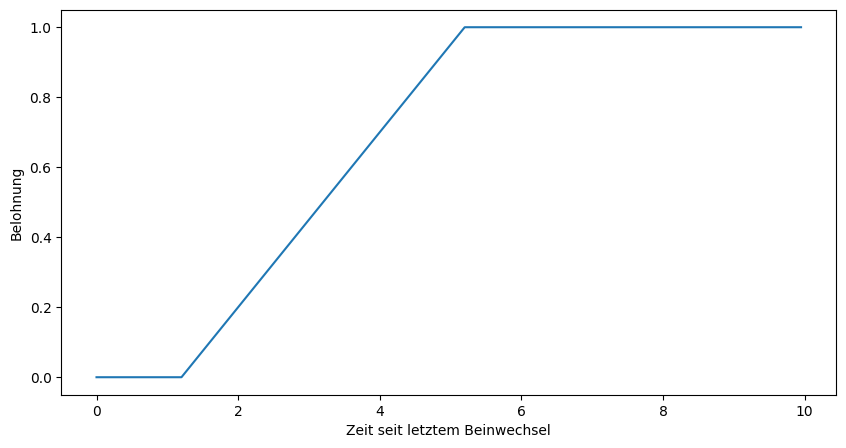
\includegraphics[width=0.9\textwidth]{img/plot_beinwechsel} 
  \caption{Beinwechsel Belohnung}
  \label{fig:plot_beinwechsel}
\end{figure}


\begin{figure}[H]
  \centering
  \begin{tabular}{ccc}
    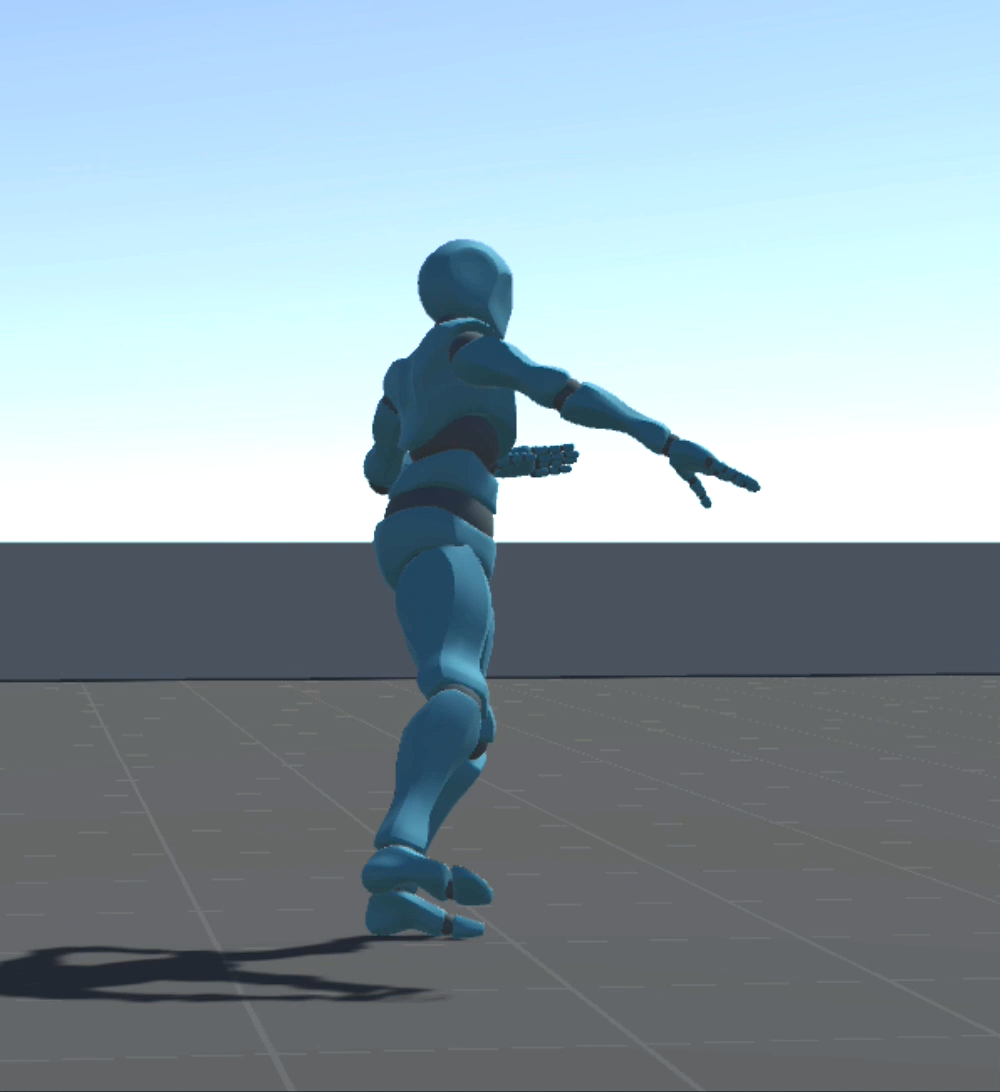
\includegraphics[width=0.27\textwidth]{img/charakter_mixamo_laufen1} & 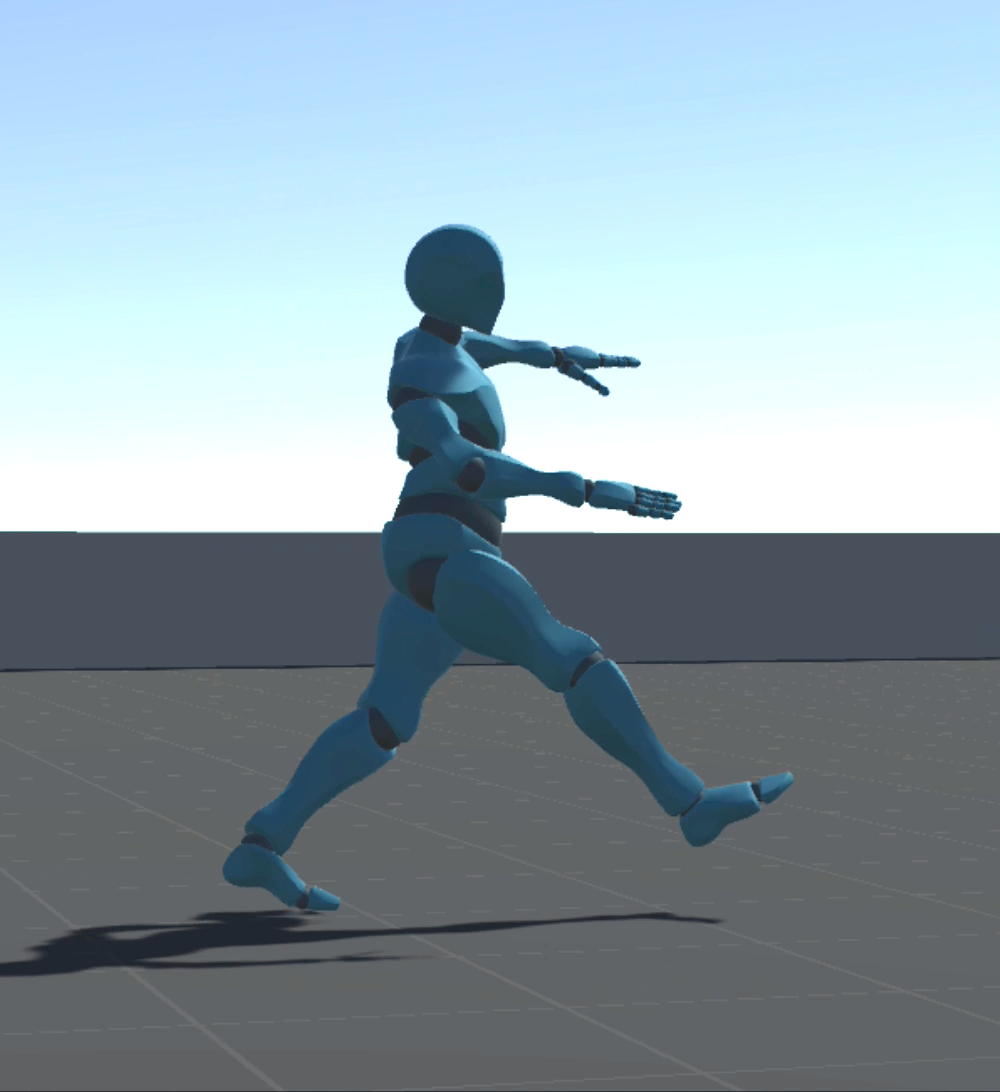
\includegraphics[width=0.27\textwidth]{img/charakter_mixamo_laufen2}  & 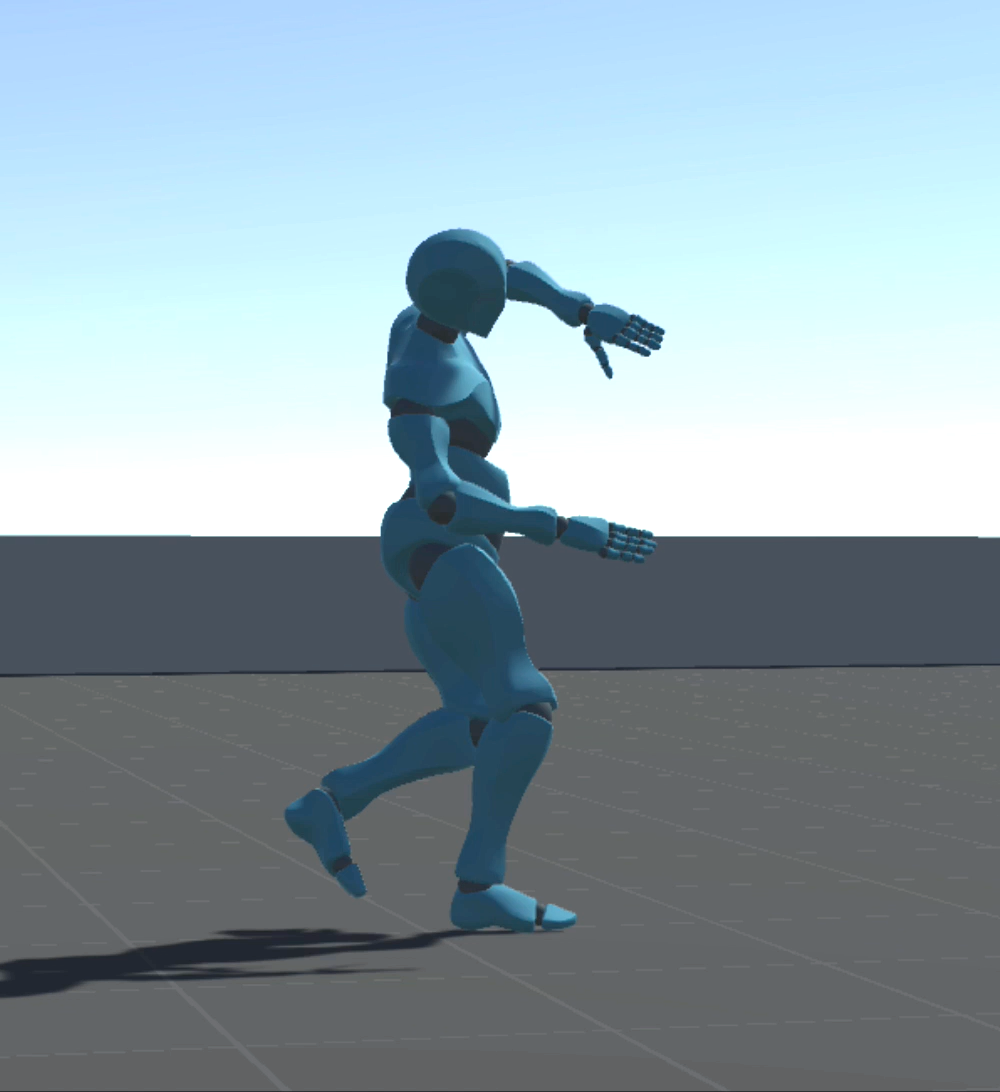
\includegraphics[width=0.27\textwidth]{img/charakter_mixamo_laufen3} \\
    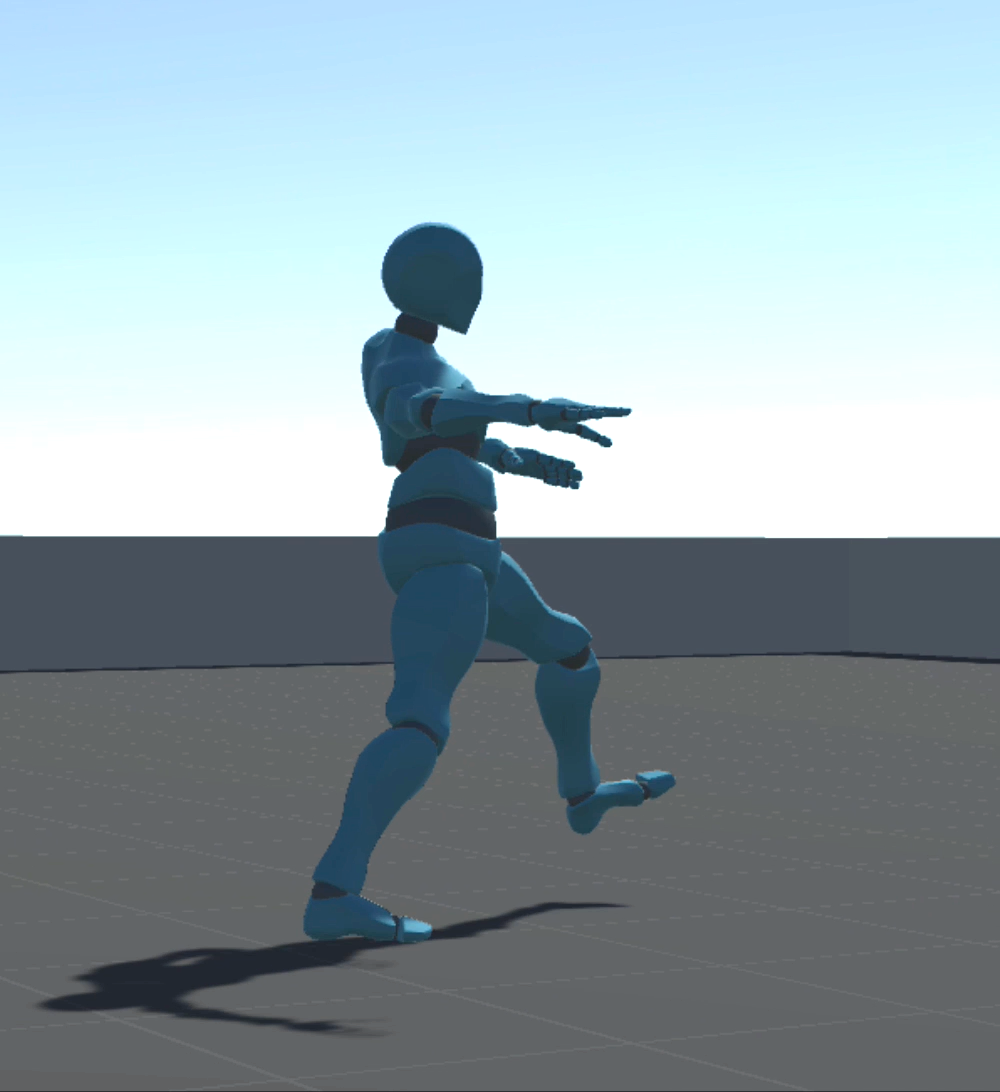
\includegraphics[width=0.27\textwidth]{img/charakter_mixamo_laufen4}  & 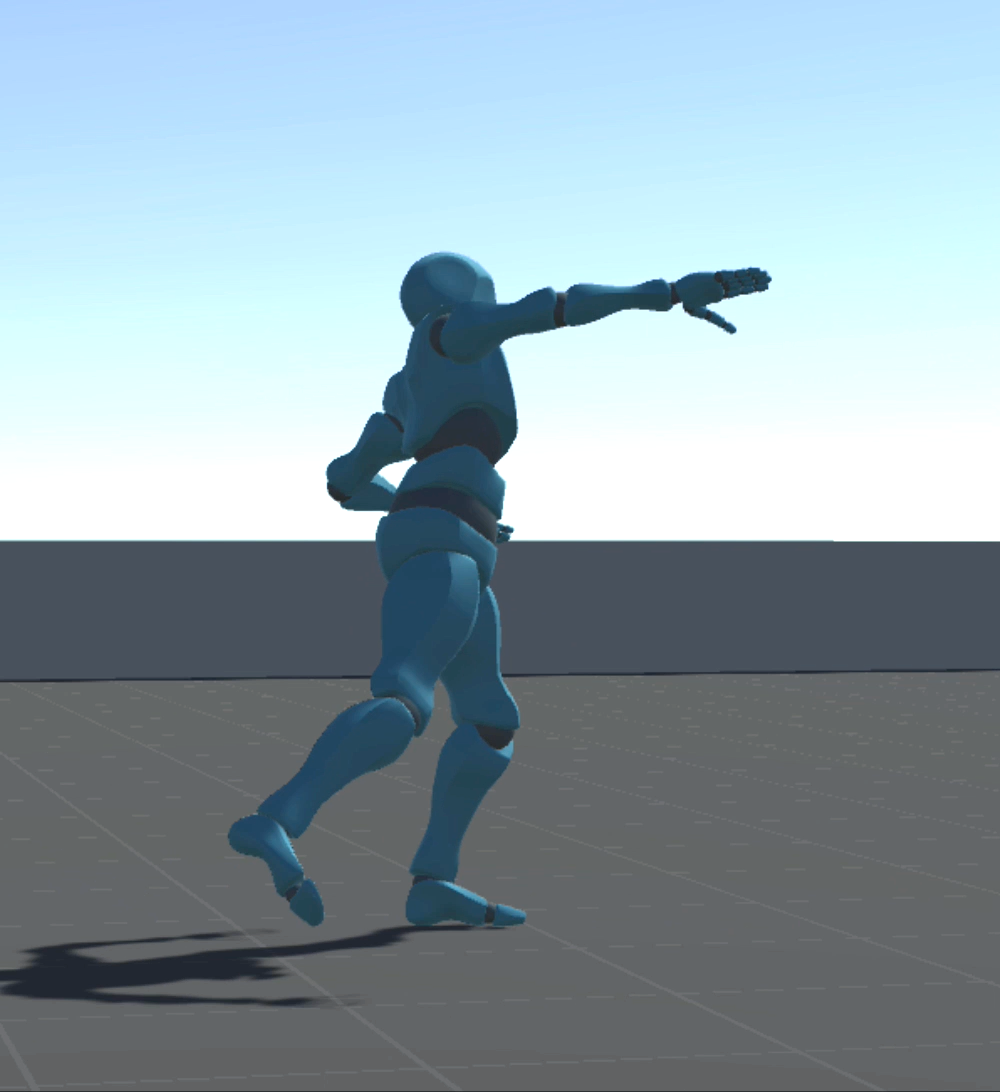
\includegraphics[width=0.27\textwidth]{img/charakter_mixamo_laufen5}  & 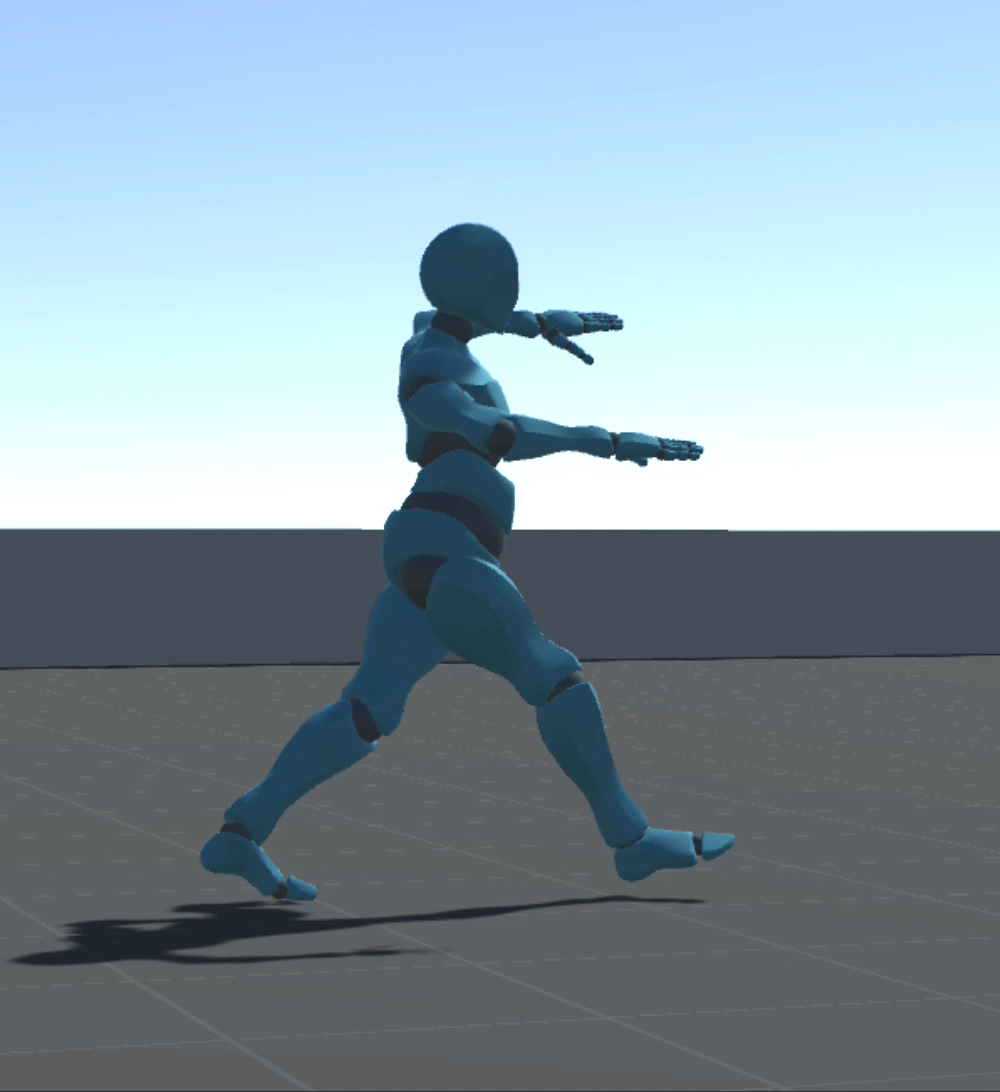
\includegraphics[width=0.27\textwidth]{img/charakter_mixamo_laufen6} \\
  \end{tabular}
  \caption{Mixamo Versuch 11 Gangbild}
  \label{fig:mixamo_versuch11_gangbild}
\end{figure}

\subsection{Belohnung für Energieminimierung}
Um das Gangbild weiter zu verbessern wird eine Belohnung eingeführt welche den Agenten belohnt wenn er so wenig wie möglich Kraft aufwendet um das Ziel zu erreichen. Genauer gesagt wird er dafür bestraft wenn die Gelenksteuerung einen zu hohe Energiekonsum aufweist.
\begin{figure}[H]
  \centering
  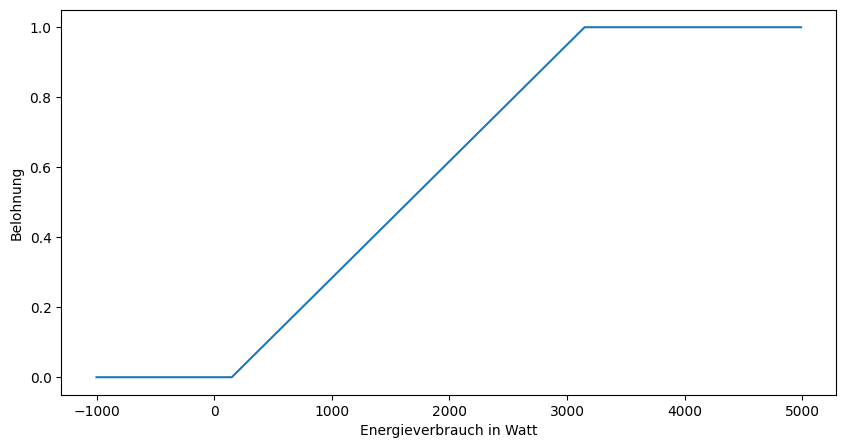
\includegraphics[width=0.9\textwidth]{img/plot_energiespar} 
  \caption{Energiespar Belohnung}
  \label{fig:plot_energiespar}
\end{figure}

\begin{figure}[H]
  \centering
  \begin{tabular}{ccc}
    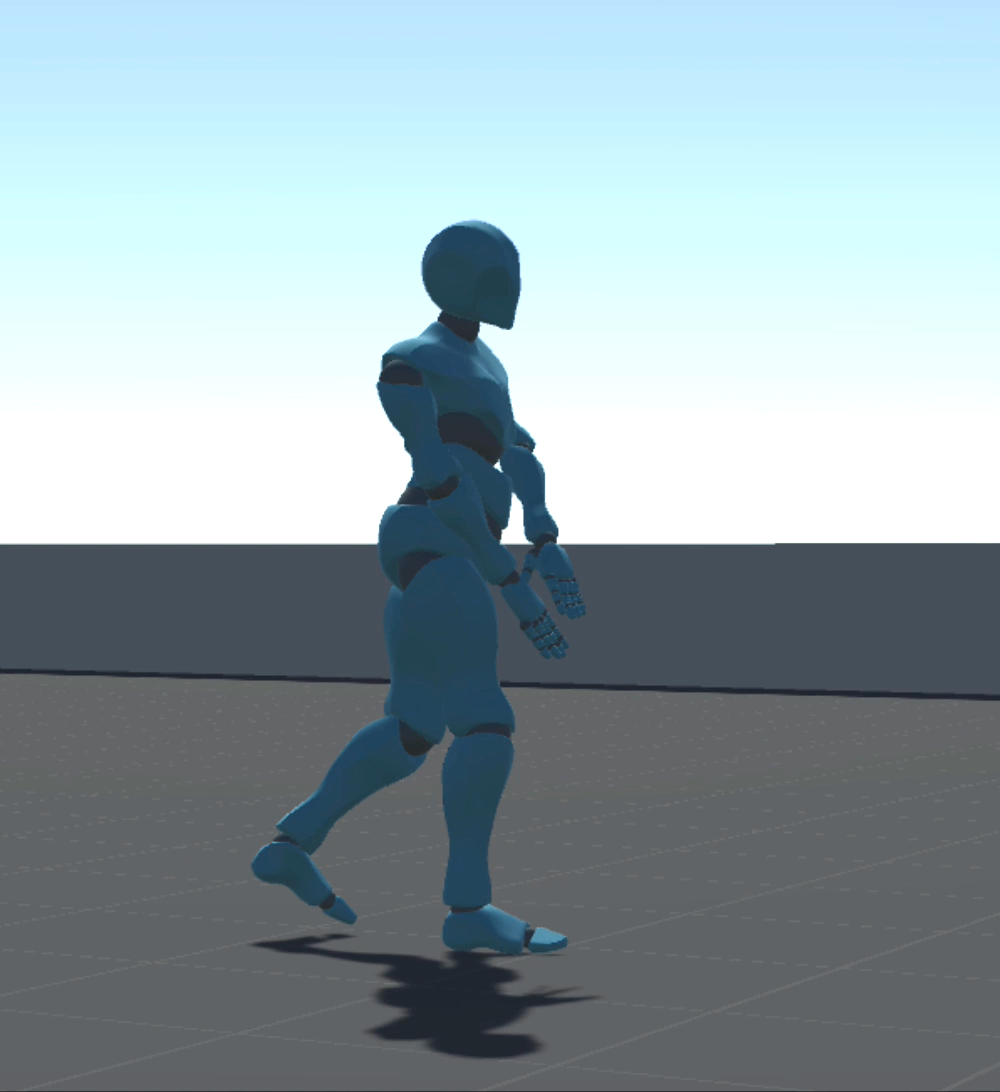
\includegraphics[width=0.27\textwidth]{img/charakter_mixamo_laufen_energiespar1} & 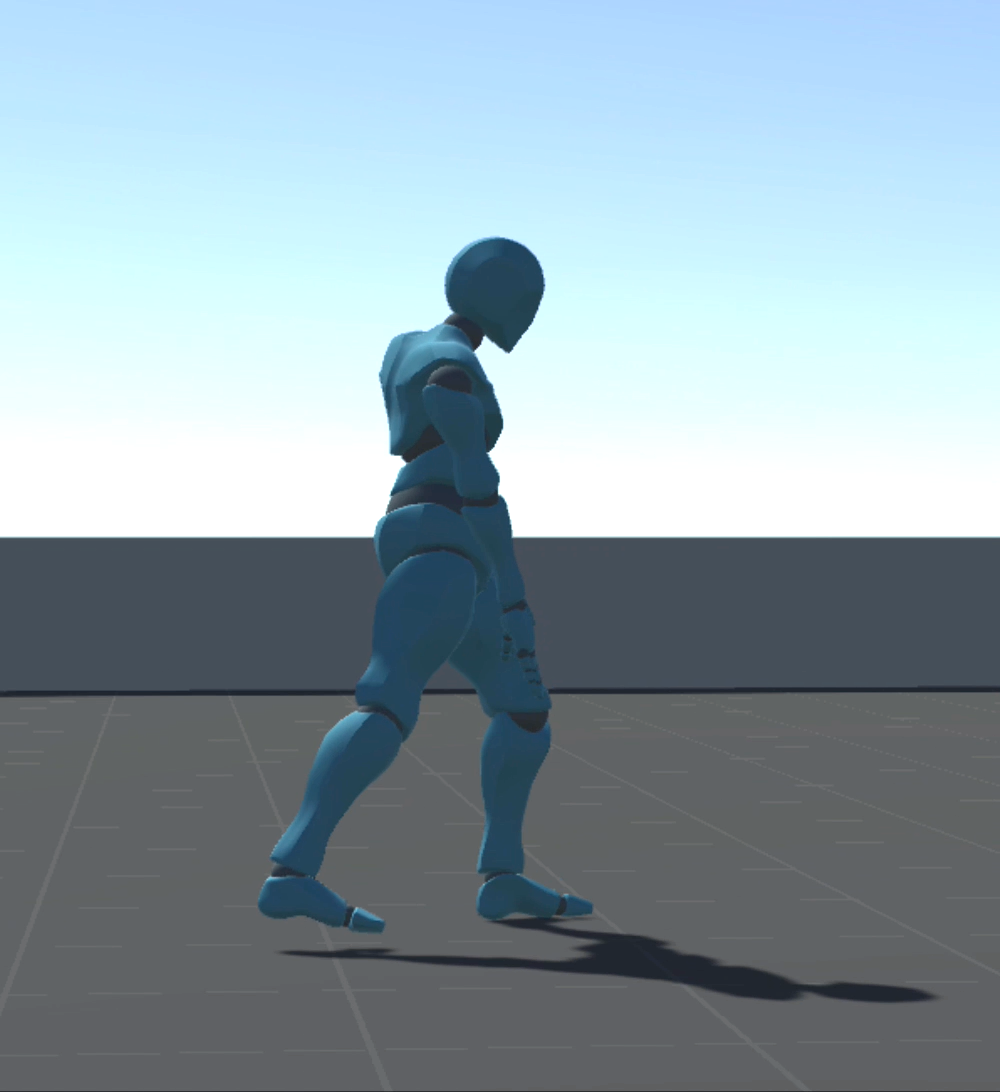
\includegraphics[width=0.27\textwidth]{img/charakter_mixamo_laufen_energiespar2}  & 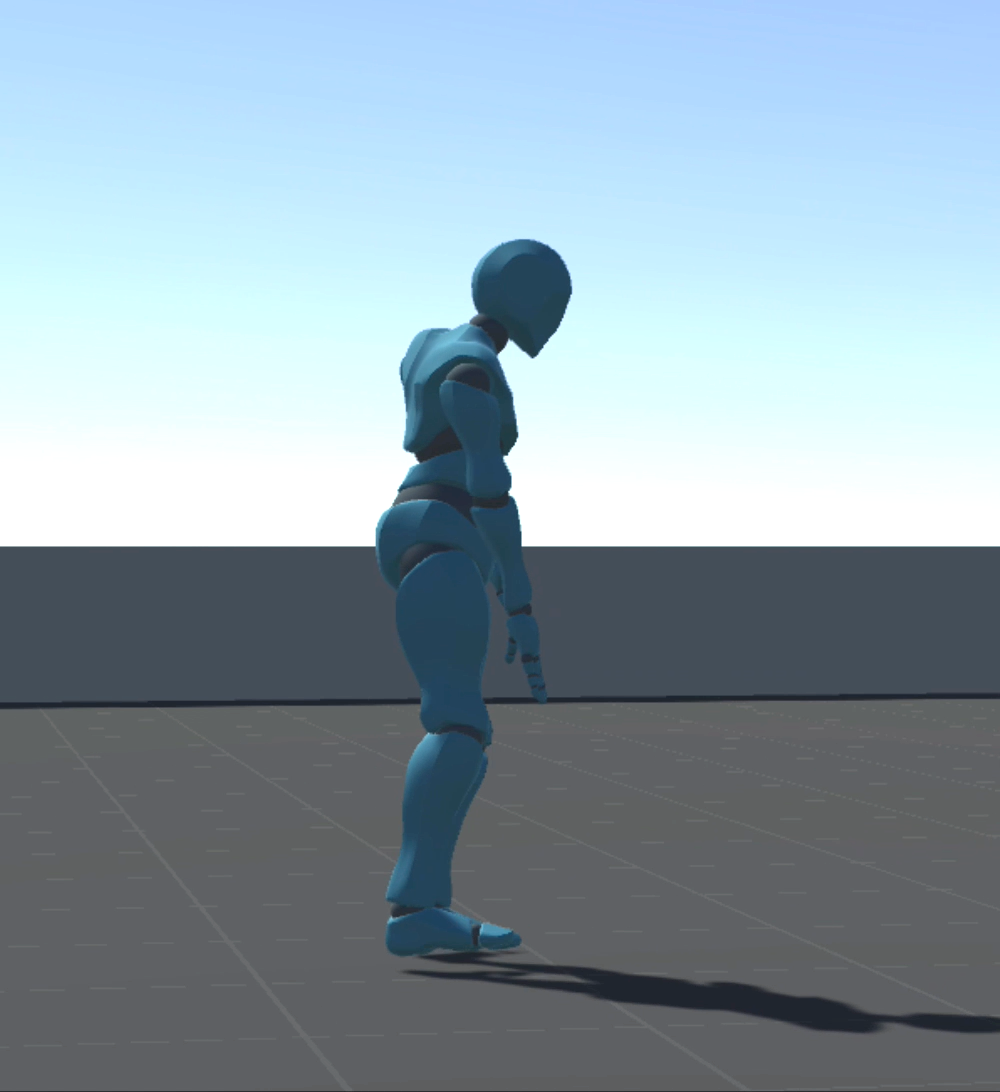
\includegraphics[width=0.27\textwidth]{img/charakter_mixamo_laufen_energiespar3} \\
    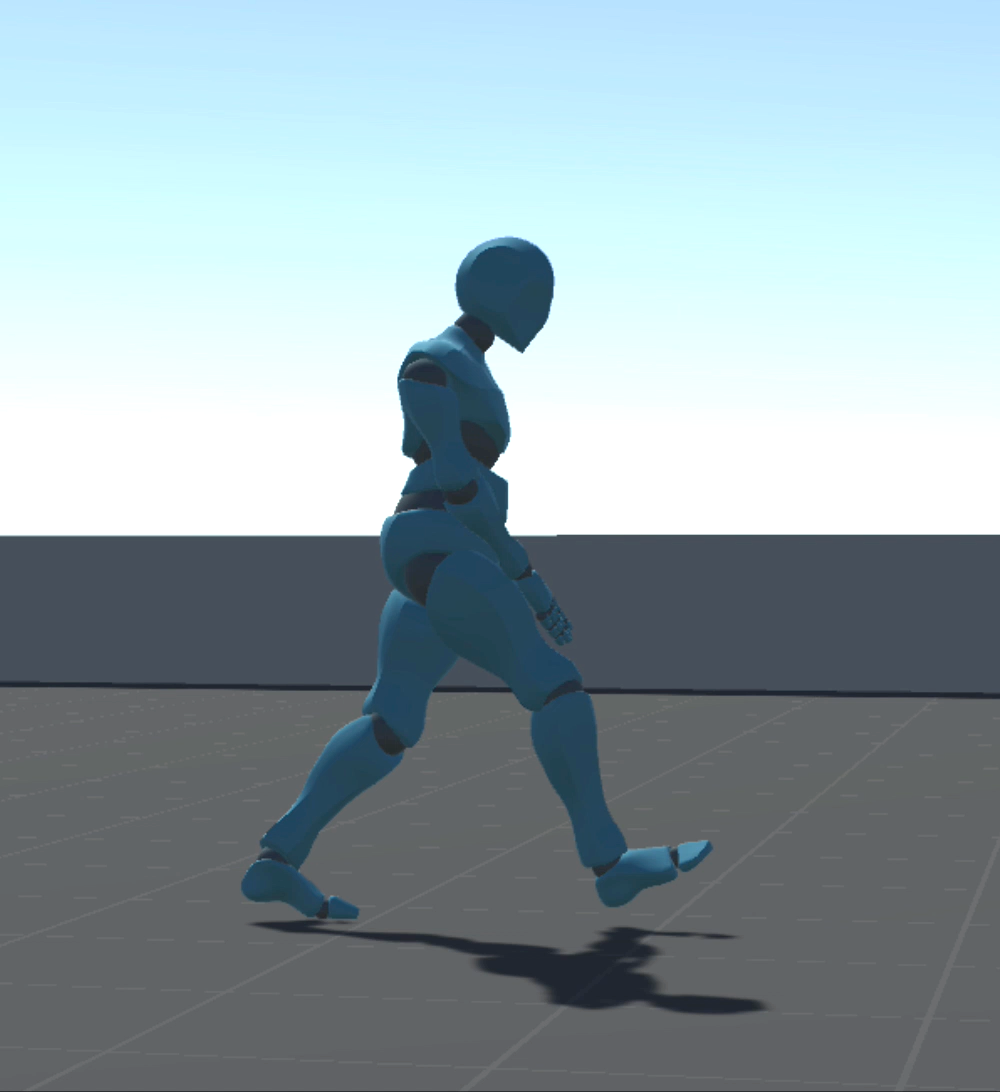
\includegraphics[width=0.27\textwidth]{img/charakter_mixamo_laufen_energiespar4}  & 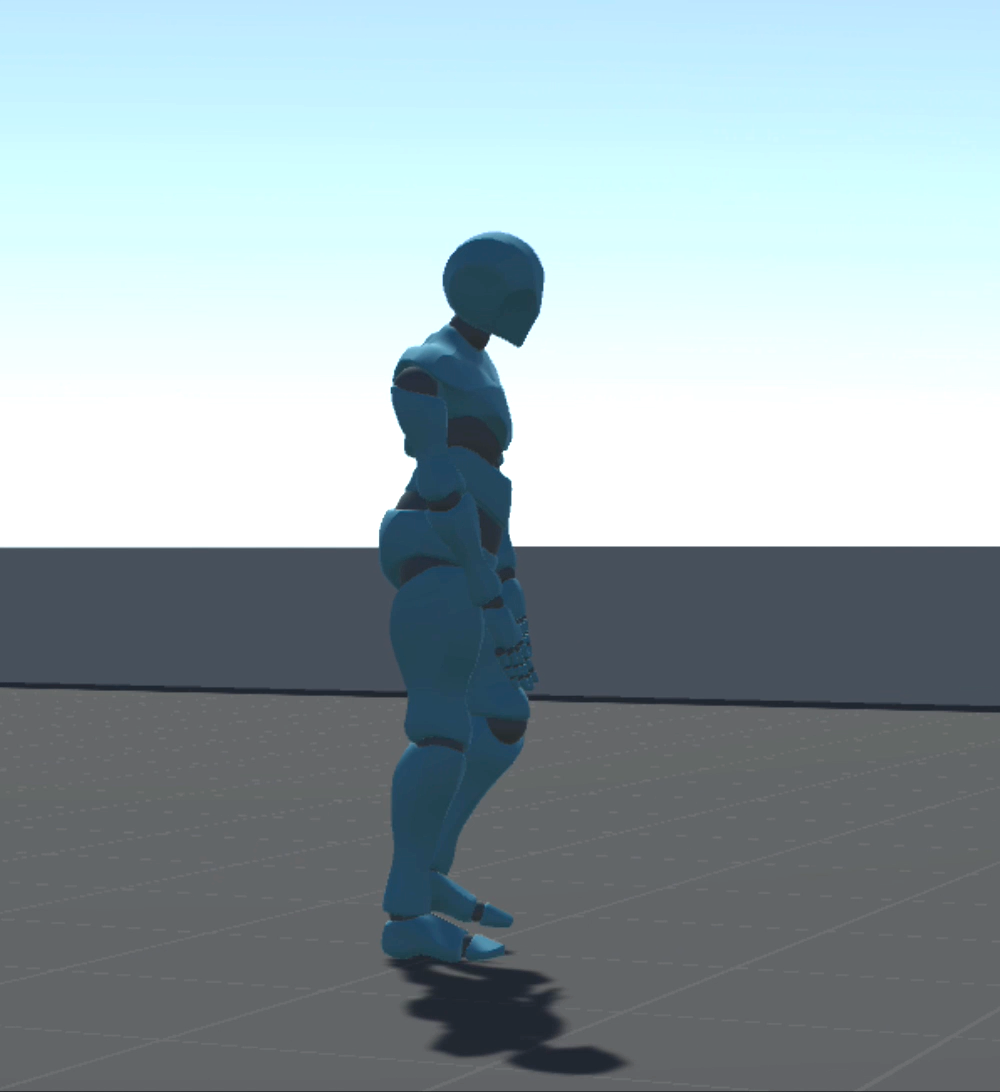
\includegraphics[width=0.27\textwidth]{img/charakter_mixamo_laufen_energiespar5}  & 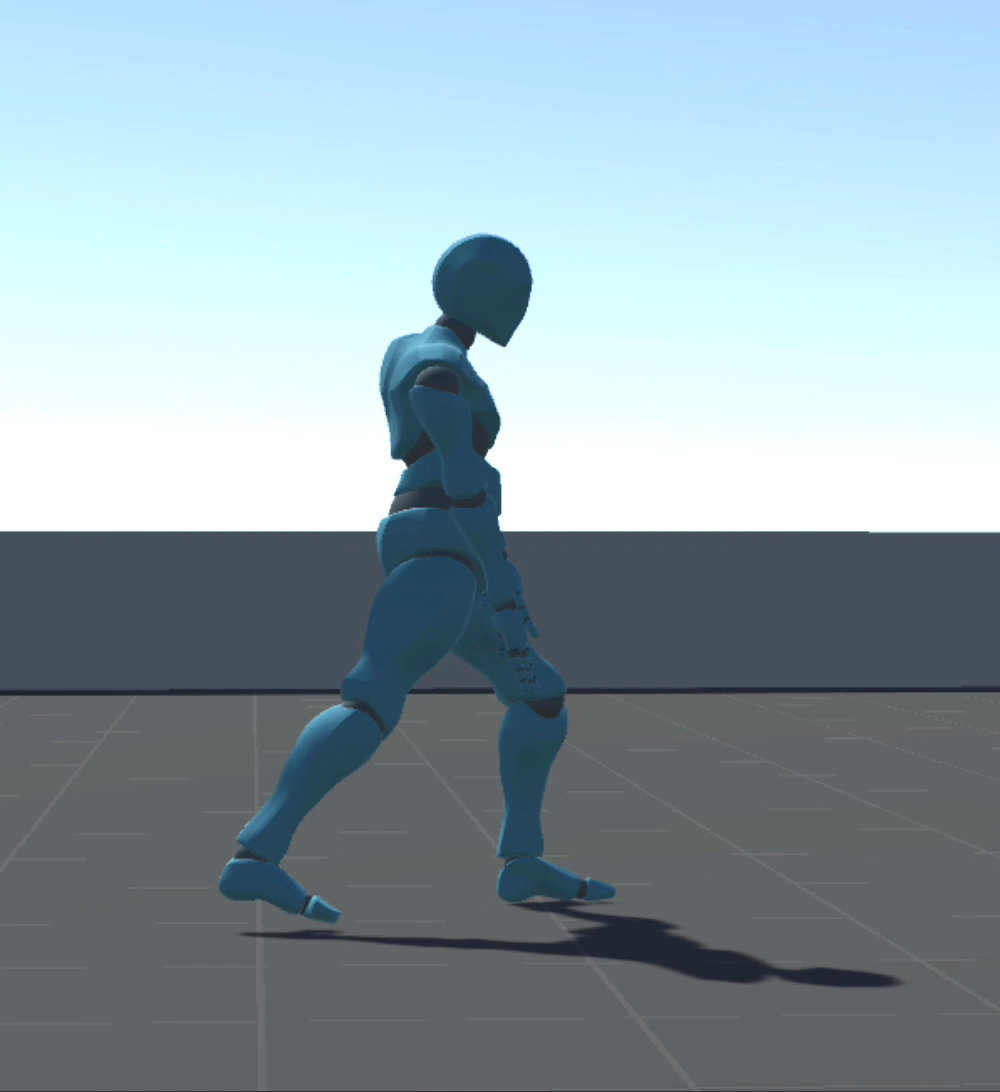
\includegraphics[width=0.27\textwidth]{img/charakter_mixamo_laufen_energiespar6} \\
  \end{tabular}
  \caption{Mixamo Versuch 12 Gangbild}
  \label{fig:mixamo_versuch12_gangbild}
\end{figure}

\subsection{Imitationslernen}